\chapter{Introduction}\label{ch_1}

The present document is a \LaTeX template for the writing up of a PhD thesis at City University London. It fulfils all the requirements established by the senate regulation 25 \citep{senate_regulation_25} and it is intended to allow the student to start the writing up straight away without worrying about the thesis format. 

Although the document obtained with this template satisfies all the university requirements for the thesis submission, it is recommended to make some test and print some example page before starting with the writing up process in order to be sure that the outcome satisfies the student. Once the full thesis is written, modifying different configurations such as the font, its size or the margins will produce undesirable effects on the floating objects' positions relative to the text.  

The typographical details of this template are summarized as follows:
\begin{enumerate}[a]
\item The size of paper used is international A4.
\item The thesis is printed on both sides of the paper.
\item Chapters always start on the right hand side page.
\item The margins are defined as: \\
	\begin{tabular}{lcr}
	inner & = & 4cm\\
	outer & = & 3cm\\
	top & = & 2.5cm\\
	bottom & = & 3cm
	\end{tabular}
\item Page numbers are located centrally at the bottom of the page, at 1.5cm above the edge. 
\item The font is the 'Computer Modern' standard font of the document class chosen for the thesis (book class).
\item The line spacing is 1.5.
\item The font normal size is set as 11pt. 
\end{enumerate}

The senate regulation 25 establishes a minimum character size of 8pt. Figure \ref{font_sizes} can be used to determine the font size to be used in the different cases.

\begin{figure}[hbtp]
\centering
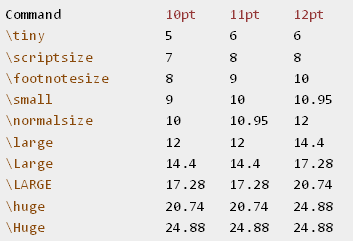
\includegraphics[width=0.6\textwidth]{Chapter_1/font_sizes}
\caption{Different font sizes depending on the chosen normal size}
\label{font_sizes}
\end{figure}

Neither headers nor footers are included in this template. However, if the student wants to include them, he/she is refereed to the 'fancyhdr' package documentation \citep{fancyhdr_doc}.\\


What follows is the 'Loren ipsum' text in order to provide a clear preview of the page layout:
\vspace{5mm}

\lipsum

